\documentclass[12pt]{article}

\usepackage[a4paper, margin=2.5cm]{geometry}
\usepackage{graphicx}
\usepackage[T1]{fontenc}
\usepackage[utf8]{inputenc}
\usepackage[hyphens]{url}

\hyphenation{
  pri-vat-nost
  ve-šta-čke
  ve-šta-čka
  in-for-ma-ci-ja
  in-for-ma-ci-je
  po-da-ta-ka
  po-da-ta-ci
  pri-vat-no-sti
  bez-bed-no-snih
  bez-bed-nost
  iden-ti-fi-ka-ci-je
  re-gu-la-tor-nih
  re-gu-la-ti-ve
  trans-pa-rent-no-sti
  al-go-ri-tam-ska
  al-go-ri-ta-ma
  mo-ne-ti-za-ci-ja
  mo-ne-ti-za-ci-je
  ma-ni-pu-la-ci-ja
  ma-ni-pu-la-ci-je
  pro-fi-li-sa-nje
  pro-fi-li-sa-nja
  in-du-stri-ja
  in-du-stri-je
  kom-pa-ni-ja
  kom-pa-ni-je
  kom-pa-ni-ja-ma
  igra-ča
  igra-či
  igra-ča-ma
  po-na-ša-nja
  po-na-ša-nje
  agre-ga-ci-ja
  agre-ga-ci-je
  te-le-me-tri-je
  te-le-me-tri-ja
}
\begin{document}

\begin{titlepage}
    \centering
    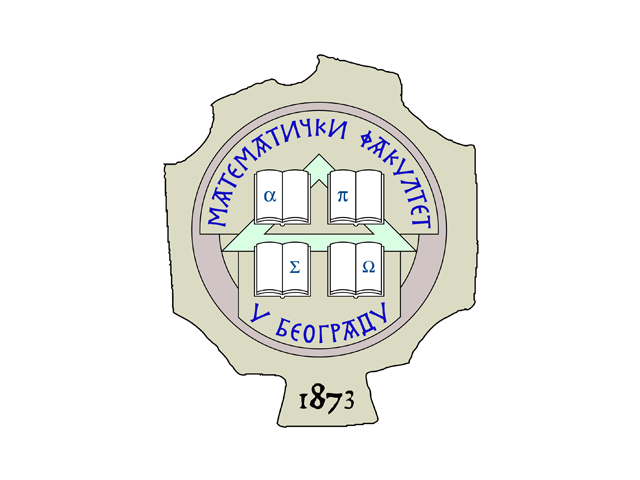
\includegraphics[width=4cm]{logo.png}\\[1cm]
    
    {\Large \textbf{UNIVERZITET U BEOGRADU}}\\[0.3cm]
    {\Large \textbf{MATEMATIČKI FAKULTET}}\\


    \vspace{0.5cm}

    \vfill

    {\LARGE \textbf{Data mining u svetu video igara: od unapređenja igre do nadzora igrača} \par}

    \vspace{3 cm}
    
    {\large Seminarski rad u okviru kursa  \par}
    {\large Računarstvo i društvo}

    \vfill

    \begin{flushleft}
        \textbf{Student:} Luka Nedeljković 147/2021\\
        \textbf{Profesor:} dr Sana Stojanović Đurđević \\
    \end{flushleft}

    \vfill

    {\large Avgust 2026 \par}

\end{titlepage}

\renewcommand{\contentsname}{Sadržaj}
\vspace{0.5cm}
\tableofcontents
\newpage
\section{Uvod}

Video igre su danas jedna od najvećih zabavnih industrija na svetu, sa prihodima koji premašuju industriju filma i muzike zajedno, i sa nekoliko milijardi igrača širom sveta \cite{kroger2023}. Iza svake partije, meča ili sesije igranja, u pozadini radi sistem koji beleži gotovo svaki potez igrača: koliko dugo igra, gde klikće, kada odustaje, koliko troši na virtuelne predmete. Ovi podaci se prikupljaju i analiziraju tehnikama koje se objedinjeno nazivaju \textit{data mining} (engl. termin za rudarenje podataka) -- otkrivanje obrazaca, korelacija i skrivenih pravilnosti u velikim skupovima podataka \cite{drachen2013}.

Data mining u igrama razvio se iz alata za unapređenje dizajna i balansiranje težine u moćan poslovni instrument: pomaže studijima da predvide kada će igrač prestati da igra, da personalizuju ponude u prodavnici koja se generiše posebno za svakog igrača, prikazujući mu baš one proizvode za koje je najverovatnije da će ih kupiti, i da otkriju varanje u realnom vremenu \cite{drachen2013}. Međutim, ista tehnologija koja unapređuje igru istovremeno omogućava neviđen nivo nadzora nad ponašanjem, navikama i čak psihološkim profilom igrača, uključujući decu koja čine značajan deo korisničke baze \cite{kroger2023}.

Ovaj rad istražuje dvostruku prirodu data mininga u video igrama: sa jedne strane kao tehniku koja unapređuje igru i industriju, a sa druge strane kao izvor ozbiljnih rizika po privatnost, autonomiju i dobrobit igrača. Detaljnija veza sa temama izučavanim u okviru kursa obrađena je u narednom poglavlju.

\subsection{Podaci kao pokretač modernih igara}

Savremene igre, naročito onlajn i mobilne, projektovane su tako da kontinuirano komuniciraju sa serverima izdavača. Svaki klik, pauza, kupovina ili poraz generiše zapis (tzv. \textit{telemetriju}) koji se šalje u analitičke sisteme \cite{drachen2013}. Za razliku od tradicionalnih, jednokratno prodatih igara iz devedesetih godina, model igre kao usluge (engl. \textit{Games as a Service}) čini da se sam proizvod neprekidno menja na osnovu onoga što podaci pokažu o ponašanju igrača. To znači da igra koju osoba igra danas nije nužno ista igra koju je igrala juče; teškoća, ponude i podsticaji se prilagođavaju u hodu, odnosno menjaju se u realnom vremenu dok igrač igra, bez potrebe da se čeka novo zvanično ažuriranje igre \cite{bourdoucen2023}.

Ova promena paradigme, od igre kao gotovog proizvoda ka igri kao platformi koja se neprekidno prilagođava korisniku, predstavlja tehnički temelj svih pitanja o privatnosti i etici koja se dalje razmatraju u ovom radu.

Dok se nekadašnja igra prodavala jednom, po fiksnoj ceni, i time je transakcija bila završena, model besplatne igre s doplatama (engl. \textit{free-to-play}) okreće logiku naopako: igra je besplatna da bi privukla što veći broj korisnika, dok se prihod ostvaruje kroz kontinuirane mikrotransakcije -- male, često ponovljene kupovine unutar same igre, poput virtuelne valute, kozmetičkih proizvoda ili dodatnog sadržaja, čija je uspešnost direktno zavisna od toga koliko dobro sistem poznaje pojedinačnog igrača \cite{drachen2013}. U takvom modelu, podatak o igraču nije sporedni nusprodukt zabave, već postaje centralna poslovna imovina studija, što objašnjava zašto se ulaganje u infrastrukturu za prikupljanje i analizu podataka u poslednjoj deceniji drastično povećalo, uporedo sa rastom prihoda od mikrotransakcija.

\section{Veza sa temama kursa}

Tema ovog rada usko je povezana sa sadržajem ovog kursa, jer se direktno nadovezuje na tri oblasti koje se u njemu izučavaju, što je detaljnije obrazloženo u nastavku poglavlja.

\textbf{Privatnost na internetu.} Rad analizira koje vrste podataka video igre prikupljaju (poglavlje~\ref{sec:tehnike}) i, u poglavlju~\ref{sec:privatnost}, pokazuje da su ti podaci, iako se to retko percipira, jednako osetljivi kao podaci koje prikupljaju pretraživači ili društvene mreže. Posebno se razmatra kako se pojedinačni, naizgled bezazleni podaci (npr. brzina reakcije ili putanja pokreta miša) mogu agregirati u detaljan profil korisnika, kao i specifičan rizik koji za privatnost predstavljaju deca i biometrijski podaci prikupljeni putem VR/AR uređaja.

\textbf{Etika u razvoju računarskih tehnologija.} Rad kritički sagledava manipulativni dizajn korisničkog interfejsa (tzv. \textit{dark patterns}, poglavlje~\ref{sec:eticki}) i monetizaciju zasnovanu na podacima o ponašanju igrača. Razmatra se etičko pitanje granice između legitimne personalizacije proizvoda i manipulacije korisnikom, kao i pitanje odgovornosti dizajnera i kompanija kada se ta granica namerno zamagljuje radi profita.

\textbf{Internet prevare i zavisnost od interneta.} Rad razmatra mehanizme poput loot boxova (engl. \textit{loot box}, virtuelnih kutija sa nasumičnim sadržajem koje se kupuju pravim novcem; poglavlje~\ref{sec:eticki}) koji ciljano koriste podatke o ponašanju igrača da bi podstakli kompulsivnu, ponekad i finansijski štetnu potrošnju, uz poređenje sa mehanikama kockanja. Ovde se nadovezuje i pitanje zavisnosti od igre kao takve, budući da se isti podaci o ponašanju koriste i za produženje vremena koje igrač provodi u igri.

\section{Data mining u video igrama -- tehnike i primena}\label{sec:tehnike}

Da bi se razumeo obim rizika i mogućnosti koje data mining donosi, potrebno je prvo razjasniti šta se tačno prikuplja i na koji način se ti podaci dalje koriste u praksi. U nastavku poglavlja prvo se razmatraju vrste podataka koje savremene igre prikupljaju, a zatim i konkretne tehnike i poslovni ciljevi koji stoje iza njihove analize.
\subsection{Vrste podataka koje igre prikupljaju}

Igre prikupljaju znatno širi spektar podataka nego što većina igrača pretpostavlja. Osim očiglednih podataka koje korisnik sam unosi (ime, datum rođenja, podaci o plaćanju), savremeni sistemi beleže i podatke generisane samom igrom: putanje kretanja lika, brzinu i preciznost reakcija, izbore u dijalozima, komunikaciju u glasovnom i tekstualnom četu, kao i podatke sa periferije poput pokreta miša, pritiska na dugmad kontrolera ili, kod VR uređaja, pokrete tela i pravac pogleda. 

Analizom ovih naizgled bezazlenih podataka mogući su zaključci koji daleko prevazilaze samu igru. Obrasci kucanja i pokreta mišem mogu otkriti biometrijski identitet korisnika, dok analiza stila igre i brzine reakcija može otkriti starost, pol, emocionalno stanje ili čak nivo stresa igrača \cite{kroger2023}. Ovakve posredne (inferencijalne) zaključke igrač retko očekuje kada pristane na prikupljanje ,,osnovnih podataka o igri``.

\subsection{Analitika igrača: zadržavanje igrača, personalizacija i sprečavanje varanja}

Sa poslovne strane, glavni cilj data mininga u igrama jeste produženje vremena koje igrač provodi u igri i povećanje njegove potrošnje. Tehnike klasterovanja koriste se da se igrači grupišu prema stilu igranja (npr. ,,agresivni``, ,,istraživački``, ,,socijalni`` tip igrača), dok se modeli mašinskog učenja koriste za predviđanje stope napuštanja igre (engl. \textit{churn}) -- trenutka kada je najverovatnije da će igrač prestati da igra, kako bi mu se pravovremeno ponudio podsticaj da ostane \cite{drachen2013}. Ovaj proces zadržavanja igrača (engl. \textit{retention}) jedan je od centralnih pokazatelja uspešnosti savremenih igara kao usluge.

Pored toga, analitika ponašanja koristi se i u svrhe koje same po sebi nisu sporne: otkrivanje varanja (engl. \textit{cheating}) u konkurentskim igrama analizom statistički neverovatnih obrazaca preciznosti ili reakcije, za šta se koriste tzv. sistemi za sprečavanje varanja (engl. \textit{anti-cheat}) -- balansiranje težine igre na osnovu agregiranih podataka o tome gde igrači najčešće odustaju, kao i unapređenje dizajna nivoa. Problem nastaje kada se ista infrastruktura koja služi ovim legitimnim ciljevima paralelno koristi za profilisanje igrača radi maksimizacije prihoda, često bez jasne granice između ta dva cilja \cite{bourdoucen2023}.
\subsection{Od sirovih podataka do poslovne odluke: kako izgleda sistem u praksi}

Tipičan analitički sistem savremene onlajn igre funkcioniše u nekoliko koraka. Prvo, klijent igre (aplikacija na telefonu, konzoli ili računaru) šalje telemetrijske događaje serveru u realnom vremenu ili u redovnim intervalima: svaki ulazak u meč, kupovina, gubitak ili napredovanje kroz nivo beleži se kao poseban zapis \cite{drachen2013}. Zatim se ti sirovi podaci agregiraju i obrađuju kroz niz automatizovanih koraka obrade velikih podataka (engl. \textit{pipeline}), gde se primenjuju tehnike klasterovanja i klasifikacije da bi se igrač svrstao u neki segment (npr. ,,igrač sa visokim rizikom od napuštanja igre`` ili ,,igrač sklon kupovini kozmetičkih proizvoda``). Konačno, na osnovu tog segmenta, sistem u realnom vremenu donosi odluku o tome koju ponudu prikazati, kada poslati notifikaciju da se igrač vrati u igru, ili da li aktivirati dodatnu proveru protiv varanja.

Ono što ovaj proces čini posebno moćnim, ali i rizičnim, jeste brzina povratne sprege: za razliku od tradicionalnih istraživanja tržišta koja traju nedeljama, sistem u igri može testirati hiljade varijacija ponude na hiljadama igrača istovremeno i u roku od nekoliko sati saznati koja varijacija donosi najveći prihod \cite{bourdoucen2023}. Ta ista infrastruktura koja omogućava brzo unapređenje igre, bez dodatnih tehničkih prepreka, može se preusmeriti i ka optimizaciji manje benignih ciljeva, poput maksimizacije vremena provedenog u igri bez obzira na dobrobit igrača.

\section{Privatnost igrača u fokusu}\label{sec:privatnost}

Pošto su vrste podataka i tehnike njihove analize razjašnjene u prethodnom poglavlju, sledeće pitanje jeste zašto ti podaci uopšte zaslužuju posebnu pažnju sa stanovišta privatnosti. Ovo poglavlje razmatra osetljivost podataka o igračima, rizike njihove agregacije, položaj dece kao posebno ranjive grupe, kao i specifičnosti biometrijskih podataka koje donose uređaji nove generacije.
\subsection{Zašto su podaci o igračima osetljivi}

Dugo se smatralo da podaci iz video igara spadaju u bezazlenu kategoriju, za razliku od, na primer, zdravstvenih ili finansijskih podataka. Kröger i saradnici osporavaju ovu pretpostavku, pokazujući da obim i granularnost podataka koje igre prikupljaju zaslužuju isti nivo pažnje kao podaci koje prikupljaju pretraživači, aplikacije za upoznavanje ili društvene mreže \cite{kroger2023}. Iz naizgled bezazlenog toka igranja mogu se izvesti zaključci o interesovanjima, ličnosti, emocionalnom stanju i potrošačkim navikama korisnika.

Poseban problem predstavlja to što igrači retko doživljavaju igru kao izvor rizika po privatnost, percepcija je da je reč o zabavi, a ne o sistemu za prikupljanje podataka, što snižava njihovu budnost u poređenju sa, recimo, korišćenjem bankarske aplikacije.
\subsection{Profilisanje i agregacija podataka}

Rizik se dodatno povećava kada se podaci iz igre kombinuju sa podacima iz drugih izvora: naloga na društvenim mrežama povezanih radi prijave, podataka o plaćanju, ili podataka sa platforme (konzole, launchera) na kojoj se igra pokreće. Agregacijom ovih izvora moguće je konstruisati profil igrača koji je detaljniji od bilo kog pojedinačnog izvora \cite{kroger2023}. Ovaj fenomen je analogan problemu agregacije podataka koji se sreće i u drugim domenima (npr. zdravstvu), ali je u igrama posebno izražen jer se retko percipira kao rizik.

Studija Burdusena i saradnika, zasnovana na analizi 21 onlajn igre i intervjuima sa 20 igrača, pokazala je da igrači imaju pogrešne pretpostavke o tome koliko se podataka zapravo prikuplja, i da je njihova spremnost da dele podatke uslovljena dizajnom igre, a ne stvarnim razumevanjem rizika \cite{bourdoucen2023}. Drugim rečima, dizajn interfejsa igre često oblikuje odluke o privatnosti više nego svesna procena igrača.
\subsection{Deca kao posebno ranjiva grupa}

Značajan deo igrača čine deca i maloletnici, što unosi dodatnu dimenziju odgovornosti. Deca su manje sposobna da prepoznaju manipulativne elemente dizajna ili da procene posledice deljenja podataka, a istovremeno predstavljaju posebno vrednu grupu za profilisanje zbog dugoročne vrednosti korisnika (engl. \textit{lifetime value}) koju studiji donose \cite{kroger2023}. Regulatori u više jurisdikcija prepoznali su ovaj problem kao prioritetan, što je detaljnije razmotreno u poglavlju~\ref{sec:pravna} kroz konkretan slučaj kompanije Epic Games.

\subsection{Biometrijski podaci i uređaji nove generacije}

Poseban izazov po privatnost predstavljaju uređaji za virtuelnu i proširenu realnost (VR/AR), kao i periferni uređaji poput naprednih kontrolera i slušalica sa mikrofonom. Kröger i saradnici posebno ističu da se iz podataka o pokretu očiju (engl. \textit{eye-tracking}), snimaka glasa i podataka sa akcelerometra mogu izvesti osetljivi zaključci koje korisnik ne očekuje, pokret očiju može otkriti fokus pažnje i kognitivno stanje, glasovni zapisi mogu otkriti emocionalno stanje ili čak zdravstvene indikatore, a podaci sa akcelerometra mogu otkriti fizičke karakteristike ili poremećaje pokreta \cite{kroger2023}.

Za razliku od podataka o klikovima ili izborima u meniju, biometrijski podaci se po prirodi ne mogu izmeniti niti ,,resetovati``, obrazac pokreta oka ili način govora ostaju karakteristika osobe tokom čitavog života, što ih čini trajno osetljivim čak i ako se konkretna igra prestane koristiti. Kako VR/AR uređaji postaju sve rasprostranjeniji, a njihovi senzori sve precizniji, količina ovakvih inferencija će verovatno rasti brže nego što regulativa i svest korisnika mogu da prate.

\section{Etički aspekti data mininga u igrama}\label{sec:eticki}

Nakon što su u prethodnom poglavlju razmotreni rizici po privatnost, prirodno se postavlja pitanje šire etičke odgovornosti industrije igara. U nastavku se razmatra kako se podaci o ponašanju igrača koriste za monetizaciju kroz loot boxove, kako se ista logika ogleda u širem spektru manipulativnih dizajnerskih rešenja (dark patterns), kao i pitanje pristanka igrača i mogućih regulatornih odgovora na ove probleme.
\subsection{Monetizacija zasnovana na podacima i loot boxovi}

Jedan od najspornijih proizvoda monetizacije zasnovane na podacima (engl. \textit{data-driven monetization}) u igrama jeste \textit{loot box} (engl. izraz za ,,kutiju s nagradom``) -- virtuelna kutija sa nasumičnim sadržajem koja se kupuje pravim novcem. Mehanika loot boxa je pažljivo optimizovana na osnovu podataka o ponašanju miliona igrača kako bi maksimizovala verovatnoću ponovljene kupovine. Istraživanje Zendla i Kernsa, zasnovano na velikom uzorku igrača, pokazalo je da postoji pozitivna korelacija između potrošnje na loot boxove i samoprijavljenih simptoma problematičnog kockanja, što loot boxove svrstava blizu granice između zabave i mehanike sličnoj kockanju \cite{zendle2018}.

Ono što loot boxove čini posebno spornim jeste da se, za razliku od tradicionalnog kockanja u kazinu gde je verovatnoća ishoda fiksna i identična za sve igrače, njihova efikasnost zasniva na kontinuiranoj analizi ponašanja igrača. Sistem prati istoriju svake pojedinačne osobe i na osnovu nje procenjuje trenutak u kome je najsklonija da izvrši kupovinu, te joj upravo tada, u realnom vremenu, prilagođava ponudu.
\subsection{Dark patterns i manipulacija ponašanjem igrača}

\textit{Dark patterns} (engl. termin za ,,mračne obrasce``) su elementi dizajna korisničkog interfejsa osmišljeni da navedu korisnika na akciju koju ne bi preduzeo da je u potpunosti razumeo posledice \cite{ftc2022}. U igrama se ovi obrasci često oslanjaju direktno na podatke o ponašanju: vremenski ograničene ponude koje se pojavljuju baš u trenutku kada je model predvideo da je igrač spreman da potroši novac, veštačka nestašica virtuelnih dobara, konfuzija oko virtuelnih valuta koja obesmišljava percepciju realne cene, kao i dugmad za kupovinu dizajnirana tako da slučajan dodir dovede do naplate.

Konkretan i dobro dokumentovan primer jeste slučaj kompanije Epic Games, izdavača igre Fortnite. Američka Federalna trgovinska komisija (FTC) je krajem 2022. godine postigla nagodbu sa kompanijom u ukupnom iznosu od 520 miliona dolara -- 275 miliona dolara zbog kršenja zakona o zaštiti privatnosti dece na internetu (prikupljanje ličnih podataka dece mlađe od 13 godina bez pristanka roditelja), i dodatnih 245 miliona dolara zbog upotrebe mračnih obrazaca dizajna koji su naveli igrače, uključujući decu, da izvrše neželjene kupovine bez jasnog pristanka. Ovo je najveća administrativna nagodba u istoriji FTC-a i predstavlja jedan od najjasnijih regulatornih priznanja da dizajn zasnovan na analizi ponašanja igrača može preći granicu iz personalizacije u manipulaciju.

Noviji radovi predlažu i sistematizaciju ovih obrazaca kroz taksonomiju sa tri dimenzije: \textit{vremensku} (npr. ograničene ponude, dnevne nagrade koje podstiču svakodnevno vraćanje u igru), \textit{novčanu} (npr. konfuzija virtuelnih valuta, loot boxovi) i \textit{socijalnu} (npr. veštački pritisak vršnjaka, isticanje da su prijatelji već kupili određeni predmet) \cite{darkpatterns2026}.

Analiza najprofitabilnijih igara sa besplatnim pristupom (engl. free-to-play) pokazuje da su ovi obrasci gušće i agresivnije zastupljeni u mobilnim igrama nego na konzolama ili računarima, upravo zato što mobilne platforme omogućavaju najpreciznije i najčešće prikupljanje podataka o trenutnom kontekstu igrača.
\subsection{Pristanak igrača i (ne)transparentnost}

Formalno, igrači daju pristanak na prikupljanje podataka prihvatanjem uslova korišćenja. U praksi, ovaj pristanak je najčešće fiktivan: politike privatnosti su duge, tehničke i retko ih igrači zaista čitaju, a dizajn interfejsa često aktivno obeshrabruje detaljniji uvid u podešavanja privatnosti \cite{bourdoucen2023}. Ovaj problem je srodan pitanju informisanog pristanka koje se sreće i u drugim oblastima primene veštačke inteligencije (npr. u zdravstvu), ali je u igrama dodatno otežan činjenicom da se igra doživljava kao zabava, a ne kao sistem koji zahteva ozbiljno razmatranje privatnosti pre upotrebe \cite{kroger2023}.
\subsection{Ko snosi odgovornost: predlozi regulatornog modela}

Pravna analiza Gudstina (Goodstein) predlaže konkretan okvir za regulaciju ovakvih praksi, umesto isključivog fokusiranja na to da li je loot box formalno igra na sreću \cite{goodstein2021}. Predlog obuhvata nekoliko elemenata: eksplicitno pravno prepoznavanje termina ,,dark pattern`` kao zasebne kategorije prekršaja, osnivanje nezavisnih tela za reviziju dizajna igara, obavezan informisani pristanak pre sprovođenja bilo kakvih istraživanja ponašanja ili psiholoških istraživanja nad korisnicima, i zabranu interfejsa dizajniranih da kod dece podstiču kompulsivno korišćenje.

Ovakav pristup je značajan jer pomera fokus rasprave sa pojedinačnog proizvoda (,,da li je loot box kockanje?") na sistemski problem (,,da li je dizajn zasnovan na podacima o ponašanju korišćen da zaobiđe racionalnu odluku korisnika?"), što je pitanje šire od same industrije igara i tiče se svake usluge koja koristi podatke o ponašanju za oblikovanje odluka korisnika.

\section{Pravna regulativa}\label{sec:pravna}

Pošto su etički problemi jasno identifikovani, logično pitanje jeste kako pravni sistemi pokušavaju da odgovore na njih. U nastavku se razmatra primena GDPR-a na video igre, konkretni primeri regulacije loot boxova u Belgiji i Sjedinjenim Američkim Državama, kao i strukturni razlozi zbog kojih nacionalna regulativa teško uspeva da isprati globalnu prirodu industrije.
\subsection{GDPR i video igre}

Opšta uredba o zaštiti podataka (engl. \textit{General Data Protection Regulation}, GDPR\footnote{\url{https://gdpr-info.eu}}), na snazi u Evropskoj uniji od 2018. godine, u potpunosti se primenjuje i na video igre kao digitalne usluge koje obrađuju lične podatke \cite{gdpr2016}. Principi minimizacije podataka i ograničenja svrhe direktno se sudaraju sa poslovnim modelom industrije igara, koja teži da prikupi što više podataka o ponašanju kako bi optimizovala angažovanje i monetizaciju.

Posebno osetljivo pitanje jeste obrada podataka maloletnih igrača, za koju GDPR (član 8) zahteva izričit pristanak roditelja za decu mlađu od 16 godina (ili niže granice, u zavisnosti od države članice). Slučaj Epic Games pokazuje da praktična primena ovog zahteva ostaje izazovna čak i za najveće kompanije u industriji \cite{ftc2022}.
\subsection{Regulacija loot boxova: Belgija i slučaj Epic Games}

Belgija je 2018. godine postala jedna od prvih zemalja koja je proglasila plaćene loot boxove oblikom nelegalnog kockanja, uz pretnju krivičnim gonjenjem izdavača koji nastave da ih nude bez licence za igre na sreću. Motivacija regulatora bila je eksplicitno usmerena na zaštitu dece od mehanika sličnih kockanju.

Međutim, naknadna analiza pokazala je da je zabrana u praksi slabo sprovedena: čak 82\% od sto najprofitabilnijih igara za iPhone u Belgiji nastavilo je da nudi neki oblik nasumične monetizacije, uključujući i 80,2\% igara namenjenih deci uzrasta 12+ godina. Ovaj nalaz pokazuje da čak i jasna zakonska zabrana nailazi na ozbiljne tehničke prepreke u primeni, kompanije mogu da prilagode ponudu na osnovu geografske lokacije korisnika (IP adrese), što otvara pitanje da li je nacionalna regulativa uopšte adekvatan nivo za rešavanje globalnog problema \cite{xiao2023}.

Nasuprot ograničenom uspehu belgijske zabrane, američki slučaj Epic Games pokazuje alternativni put, direktnu novčanu sankciju i strukturne promene u dizajnu proizvoda, umesto potpune zabrane mehanike. Ova dva pristupa: evropski (zabrana kroz zakone o kockanju) i američki (sankcionisanje kroz zaštitu potrošača i dece) ilustruju da još uvek ne postoji usaglašen globalni regulatorni model za monetizaciju zasnovanu na podacima u igrama.
\subsection{Zašto je nacionalna regulativa nedovoljna}

Oba prethodno opisana slučaja dele istu strukturnu slabost: video igre su globalni proizvod, dok je regulativa i dalje uglavnom nacionalna ili regionalna. Slučaj Belgije pokazao je da kompanije mogu tehnički prilagoditi ponudu na osnovu geografske lokacije korisnika, čime jedna jurisdikcija sama po sebi teško može da nametne standard koji se ne zaobilazi jednostavnim sredstvima poput VPN-a. S druge strane, čak i snažna sankcija poput one protiv Epic Gamesa deluje tek nakon što je šteta već nastala, kao reaktivna, a ne preventivna mera. Iz ovoga proizlazi da efikasna zaštita igrača verovatno zahteva kombinaciju pristupa: jasne tehničke standarde na nivou industrije (poput onih koje predlaže Gudstin), regulativu usklađenu na nivou više država (po uzoru na GDPR unutar EU), i alate koji omogućavaju roditeljima i samim igračima da samostalno ograniče izloženost monetizaciji zasnovanoj na podacima.

\section{Ključni radovi}
\subsection{Kröger i dr. (2023) -- Nadzor nad igračima}

Rad Jakoba Leona Krögera i saradnika, \textit{Surveilling the Gamers: Privacy Impacts of the Video Game Industry}, objavljen u časopisu \textit{Entertainment Computing} \cite{kroger2023}, predstavlja glavni teorijski oslonac ovog seminarskog rada. Autori nude sistematsku klasifikaciju vrsta podataka koje video igre prikupljaju i, oslanjajući se na patente i literaturu iz više disciplina, pokazuju kako naizgled bezazleni podaci o igranju mogu otkriti biometrijski identitet, starost, pol, emocije, veštine, interesovanja i crte ličnosti korisnika. Vrednost ovog rada za temu seminarskog leži upravo u tome što po prvi put sistematski argumentuje da industrija igara zaslužuje isti nivo istraživačke i regulatorne pažnje kao i drugi digitalni servisi koji se tradicionalno smatraju rizičnijim po privatnost.
\subsection{Burdusen i dr. (Bourdoucen et al., 2023) -- Cena privatnosti}

Rad Amel Burdusen, Lejsan Nurgalijeve i Jane Lindkvist, \textit{Privacy Is the Price: Player Views and Technical Evaluation of Data Practices in Online Games}, objavljen na konferenciji ACM CHI PLAY 2023 \cite{bourdoucen2023}, odabran je kao drugi ključni rad zbog toga što kombinuje tehničku analizu prakse (21 onlajn igra) sa empirijskim uvidom u perspektivu samih igrača (20 intervjua). Za razliku od isključivo teorijskog pristupa, ovaj rad pokazuje da spremnost igrača da dele podatke zavisi od konteksta i dizajna igre, a ne od stvarnog razumevanja rizika, čime direktno potkrepljuje centralnu tezu rada o ulozi manipulativnog dizajna u prikupljanju podataka. Autori dodatno nude i konkretne preporuke za dizajn, veću transparentnost i mogućnost odustajanja od invazivnog prikupljanja podataka.

\section{Zaključak}

Data mining je postao neodvojiv deo savremenog dizajna i poslovanja video igara. Iste tehnike koje omogućavaju otkrivanje varanja, balansiranje težine i unapređenje korisničkog iskustva, koriste se i za profilisanje igrača i optimizaciju monetizacije na način koji igrač retko u potpunosti razume ili na koji zaista pristaje. Ovaj rad je pokazao da podaci iz igara nisu bezazlena kategorija; oni omogućavaju zaključke o identitetu, ponašanju i emocionalnom stanju korisnika koji su uporedivi sa rizicima poznatijim iz drugih digitalnih usluga.

Na etičkom planu, primeri poput loot boxova i slučaja Epic Games pokazuju da granica između legitimne personalizacije i manipulativnog dizajna često zavisi od toga koliko transparentno je igraču predstavljeno na čemu se ponuda zasniva. Regulativa, bilo kroz zakone o kockanju (Belgija) ili kroz zaštitu potrošača i dece (SAD), pokušava da odgovori na ovaj problem, ali primeri pokazuju da sprovođenje zaostaje za tempom kojim industrija razvija nove, sve suptilnije tehnike zasnovane na podacima.

Otvorena pitanja ostaju: da li igrač uopšte može dati smislen pristanak na prikupljanje podataka u sistemu koji je namerno projektovan da bude zabavan i nezahtevan za pažnju? Da li je nacionalna regulativa dovoljna za industriju koja posluje globalno i može tehnički da prilagodi ponudu po državi? I konačno, ko snosi odgovornost kada je granica između dobrog dizajna igre i manipulacije ponašanjem igrača namerno zamagljena? Odgovor na ova pitanja zahteva saradnju dizajnera igara, istraživača privatnosti i regulatora, jer nijedna od ove tri strane sama ne može da reši problem koji je istovremeno tehnički, poslovni i etički.

Važno je naglasiti da data mining sam po sebi nije problem, tehnike opisane u ovom radu omogućavaju i mnoge korisne stvari: bolje balansirane igre, efikasnije otkrivanje varanja i personalizovano iskustvo koje mnogi igrači cene. Problem nastaje kada se ista infrastruktura, bez transparentnosti prema korisniku, preusmeri ka ciljevima koji nisu u interesu igrača, poput podsticanja kompulsivne potrošnje kod dece ili konstruisanja detaljnih profila bez njihovog znanja. Budući razvoj industrije, naročito širenje VR/AR uređaja sa sve preciznijim senzorima, čini da ovo pitanje postaje sve hitnije, a ne manje relevantno, uprkos tome što video igre i dalje uglavnom ostaju van glavnog fokusa javne rasprave o privatnosti u poređenju sa društvenim mrežama i pretraživačima.

\renewcommand{\refname}{Literatura}

\begin{thebibliography}{99}

\bibitem{drachen2013}
A. Drachen, C. Thurau, J. Togelius, G. N. Yannakakis, C. Bauckhage, ``Game Data Mining,'' in \textit{Game Analytics}, Springer, London, 2013, pp. 205--253. DOI: \url{https://doi.org/10.1007/978-1-4471-4769-5_12}

\bibitem{kroger2023}
J. L. Kröger, P. Raschke, J. Percy Campbell, S. Ullrich, ``Surveilling the Gamers: Privacy Impacts of the Video Game Industry,'' \textit{Entertainment Computing}, vol. 44, 2023, Art. no. 100537. DOI: \url{https://doi.org/10.1016/j.entcom.2022.100537}

\bibitem{bourdoucen2023}
A. Bourdoucen, L. Nurgalieva, J. Lindqvist, ``Privacy Is the Price: Player Views and Technical Evaluation of Data Practices in Online Games,'' \textit{Proceedings of the ACM on Human-Computer Interaction}, vol. 7, no. CHI PLAY, 2023, pp. 1136--1178. DOI: \url{https://doi.org/10.1145/3611064}

\bibitem{zendle2018}
D. Zendle, P. Cairns, ``Video game loot boxes are linked to problem gambling: Results of a large-scale survey,'' \textit{PLoS ONE}, vol. 13, no. 11, 2018, e0206767. DOI: \url{https://doi.org/10.1371/journal.pone.0206767}

\bibitem{xiao2023}
L. Y. Xiao, ``Breaking Ban: Belgium's Ineffective Gambling Law Regulation of Video Game Loot Boxes,'' \textit{Collabra: Psychology}, vol. 9, no. 1, 2023, Art. no. 57641. DOI: \url{https://doi.org/10.1525/collabra.57641}

\bibitem{ftc2022}
Federal Trade Commission, ``Fortnite Video Game Maker Epic Games to Pay More Than Half a Billion Dollars over FTC Allegations of Privacy Violations and Unwanted Charges,'' Press Release, Dec. 19, 2022. Dostupno na: \url{https://www.ftc.gov/news-events/news/press-releases/2022/12/fortnite-video-game-maker-epic-games-pay-more-half-billion-dollars-over-ftc-allegations}

\bibitem{gdpr2016}
Evropski parlament i Savet Evropske unije, ``Uredba (EU) 2016/679 o zaštiti fizičkih lica u vezi sa obradom podataka o ličnosti i o slobodnom kretanju takvih podataka (Opšta uredba o zaštiti podataka -- GDPR),'' \textit{Službeni list Evropske unije}, L 119, str. 1--88, 2016. Dostupno na: \url{https://gdpr-info.eu}

\bibitem{goodstein2021}
S. Goodstein, ``When the Cat's Away: Techlash, Loot Boxes, and Regulating `Dark Patterns' in the Video Game Industry's Monetization Strategies,'' \textit{University of Colorado Law Review}, vol. 92, no. 1, pp. 285--336, 2021. Dostupno na: \url{https://scholar.law.colorado.edu/lawreview/vol92/iss1/6/}

\bibitem{darkpatterns2026}
S. Gutiérrez-Manjón, S. Gómez-García, G. Bonales-Daimiel, ``Designing for monetization: A taxonomy of dark patterns in top-grossing GaaS video games,'' \textit{Tripodos}, no. 59, pp. 76--97, 2026. DOI: \url{https://doi.org/10.51698/tripodos.2026.59.05}

\end{thebibliography}

\end{document}
